\chapter{Of Users and Groups}
\label{chap:multi-user}

\begin{quote}

{\em We trust you have received the usual lecture from
the local System Administrator. It usually boils down
to these three things:\\
\#1) Respect the privacy of others.\\
\#2) Think before you type.\\
\#3) With great power comes great responsibility.} \\
-- Output of {\tt sudo(8)} upon first invocation.
\end{quote}

% XXX add graphic
%\begin{figure}[hb]
	%\raggedleft
	%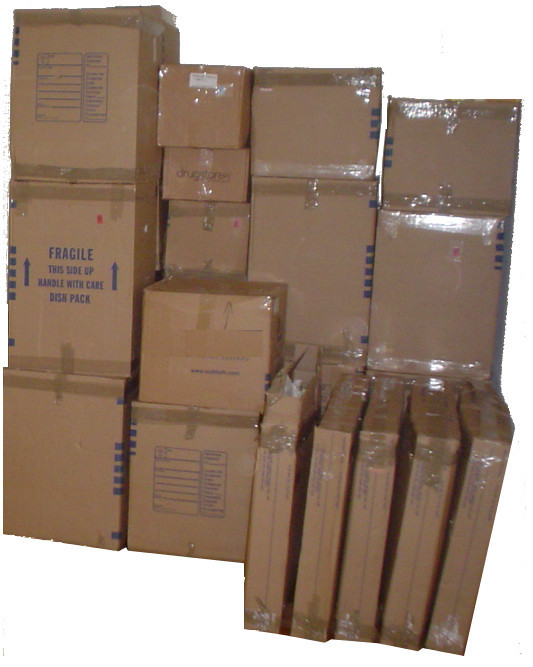
\includegraphics[width=.25\textwidth]{05/pics/many-boxes}
%\end{figure}

\section{Introduction}
\label{multi-user:introduction}

As was noted in Section \ref{unix:basics:multi}, Unix
was designed as a multi-tasking, {\em multi-user}
system, allowing simultaneous access by different
people.  This concept, also found in all of today's
mainstream operating systems as well, demands
important safeguards to prevent both accidental as
well as intentional (i.e. malicious) access by
unauthorized parties.  Since this property affects
virtually all aspects of system administration --
ranging from account management to the way different
software components interact with one another -- it is
important to fully understand the implications of the
nature of a multi-user system.

In this chapter, we will discuss the different types
of users and groups as well as talk about user
authentication on our systems.  Note that even though
there are many parallels to authentication by remote
clients against a service we may offer (such as users
logging into our website), in this chapter we restrict
ourselves to the ``local'' systems and how we access
them internally.

Even if you are comfortable with the Unix multi-user
model, you may still find that explicitly identifying
its inherent requirements and trust models will help
in formalizing your access control requirements so
as to express and apply them using your configuration
management system\index{Configuration Management}, as
discussed in the Chapter
\ref{chap:configuration-management}.

As one of our Pillars of Exceptional System Design,
the topic of security weaves through this book like a
red thread, and multi-user principles and the
implications of different access- and trust levels
necessitate a look ahead at topics and ideas discussed
in more detail in Chapter
\ref{sec:security:authn-authz}.  Hence, discussing
the core concepts of {\em
authentication}\index{authentication} and {\em
authorization}\index{authorization} is a natural
requirement and we will attempt to broadly cover them
in this chapter as well.  But let's not get ahead of
ourselves...


\section{Types of Users}
\label{multi-user:types}
\index{Accounts, Types of}

Allowing more than one person access to the resources
of a system requires the computer to be able to {\em
distinguish} between different users, which of course
is done by providing distinct {\em user accounts}.
When a user wishes to use the system, she identifies
herself to the computer (for example by entering her
login name), upon which the system authenticates her
(for example by prompting her for a password). Upon
successful authentication, she is then granted access
to her files and/or is allowed to run certain
programs.  But this simple association of human beings
to computer accounts -- in the Unix world implemented
using numeric {\em user-IDs} -- does not paint a
complete picture.

It is easy to assume that different ``users'' refer to
distinct people accessing the resources, and ideally
we'd want to keep the mapping between the two sets
(``persons'', ``accounts'') to be of a 1-to-1 (and
{\em onto}) nature.  But we quickly run into problems:

On a typical Unix system, you will find a perhaps
surprising number of accounts that are {\em not}
associated with actual human beings at all. To
illustrate this, Listing \ref{code:cat-passwd}
displays excerpts of the standard Unix password
database, the {\tt /etc/passwd} file, on a NetBSD
system.  Reviewing the first few rows, we find most of
them reference so-called {\em system
accounts}\index{Accounts, System}, present to allow
specific services to run with only the permissions
they need, a concept known as privilege
separation\index{privilege separation} or the
{\em Principle of Least Privilege}\index{Least Privilege,
Principle of}. This ensures, for example, that a
software error in one d\ae mon cannot accidentally
lead to access or deletion of files owned by another
user.

\begin{lstlisting}[float,label=code:cat-passwd,caption={Excerpt of a
typical {\tt /etc/passwd} file on a NetBSD system\index{\tt apache}}]
root:*:0:0:Charlie &:/root:/bin/csh
toor:*:0:0:Bourne-again Superuser:/root:/bin/sh
daemon:*:1:1:The devil himself:/:/sbin/nologin
bin:*:3:7:Binaries Commands and Source:/:/sbin/nologin
postfix:*:12:12:& pseudo-user:/var/spool/postfix:/sbin/nologin
named:*:14:14:& pseudo-user:/var/chroot/named:/sbin/nologin
ntpd:*:15:15:& pseudo-user:/var/chroot/ntpd:/sbin/nologin
sshd:*:16:16:& pseudo-user:/var/chroot/sshd:/sbin/nologin
_pflogd:*:18:18:& pseudo-user:/var/chroot/pflogd:/sbin/nologin
nobody:*:32767:39:Unprivileged user:/nonexistent:/sbin/nologin
www:*:1003:1000:apache www user:/nonexistent:/sbin/nologin
spamd:*:1004:1001:Spamd User:/var/chroot/spamd:/sbin/nologin
deploy:*:1234:1234:& User:/var/app:/usr/local/bin/app-update
jschauma:*:1000:100:Jan Schaumann:/home/jschauma:/bin/ksh
alice:*:1001:100:Vincent Damon Furnier:/home/alice:/bin/ksh
bob:*:1007:100:Nesta Robert Marley:/home/bob:/bin/sh
\end{lstlisting}

In addition to these system accounts, we also
frequently find what has become to be known as {\em
role accounts}\index{Accounts, Role}: accounts that,
while not specifically tied to a single person, are
used to allow multiple people to initiate certain
well-defined actions.  A common example is a role
account to allow for automated updates to a given
service or application. \\

In order to manage the resources to be made available
to different users, to control the system, to add or
remove software etc., we require the use of an
omnipotent account, known as the
superuser\index{superuser}.  This account is commonly
called the {\tt root} account, and is identified by
the numeric user-ID 0.\footnote{As user privileges
on a Unix system are only identified by the {\em
effective user-ID} of a given process, the system does
not care one bit whether or not the string mapped to
the UID 0 happens to be ``root'' or ``bob'' or
``susan''. That is, superuser accounts with other
names are entirely possible; ``root'' just happens to
be one of those old Unix conventions we've all grown
so accustomed to.  It is good practice -- and part of
most standard security scans -- to periodically check
for the existence of ``other'' accounts with UID 0.}
In order to gain superuser privileges, a user needs to
either log in as {\tt root}, assume the superuser's
identity via the {\tt su(1)}\index{\tt su(1)}
command, or make use of, for example, the popular {\tt
sudo(8)}\index{\tt sudo(8)} utility (which also
offers some more fine-grained control over who may
gain what privileges).

\begin{sidenote}
{\bf Of Headless Users and Privilege} \\

{\em Role Accounts} may be known by a variety of
names, depending on the history of the organization:
``service account'', ``headless users'' (because no human is
associated with the account), or, frequently, by the
name of the company or organization.  Now a funny
side-effect of using a service account intended for
privilege separation to automate certain tasks is
that this account becomes more and more powerful with
time: every task it needs to accomplish (such as
installing or updating software, starting or stopping
services, monitoring services or alerting on
conditions) requires the user to have the necessary
privileges. \\ [10pt]

Take a look in your {\tt /etc/passwd} -- if you work
at company ``Gizmo App, Inc.'', chances are the most
powerful user (besides {\tt root}, of course) is
``gizmo'', and {\tt gizmo}'s access credentials are
shared across multiple systems.  We will discuss this
dilemma and some possible ways to mitigate it in
Chapter \ref{chap:security}.
\end{sidenote}


Perhaps somewhat paradoxically -- usually, we wish to
have a unique mapping from exactly one person to
exactly one user-ID -- access to this superuser
account is shared: all system administrators within an
organization need to have this kind of access by
necessity.\footnote{A discussion of the limitations in
the traditional Unix permissions model that make this
shared superuser account a virtual necessity would be
beyond the scope of this chapter.  For completeness's
sake, however, we should mention that more modern
access semantics, such as {\em mandatory access
controls} (MAC), {\em role-based access controls}
(RBAC), or POSIX ``capabilities''  can been added,
albeit at the cost of increased complexity.}

Reviewing these access rules, we can identify mappings
of zero, one or more people to a given account (Figure
\ref{fig:multi-user:mappings}), as well as a single
person with access to multiple accounts.  From the
system's perspective the differences are irrelevant
(all process privileges are granted solely based on
the UID), but as system administrators, we have to
treat each class of users differently.  As a general
rule of thumb, we want to ensure, for example, that
only those accounts used by people have an
interactive login session.  All other accounts should
be restricted such that they can only execute specific
commands or access specific files\footnote{On some
Unix systems, it is possible to restrict a given
process to a specific subset of the file system --
see, for example, the {\tt chroot(8)}\index{\tt
chroot(8)} command.  In the past, assigning a user a
so-called {\em restricted} shell was another method of
limiting what actions a user may perform.}.  This
becomes difficult quickly especially when using role
accounts, as often a certain set of interactive
commands need to be allowed.  Care must be taken to
correctly identify and enforce the restriction to
just these commands.

If you look closely at the example password file shown
in Listing \ref{code:cat-passwd}, you may notice that
in addition to the {\tt root} account there is a
second account with UID 0, called {\tt toor}. This
account, often found on the BSD derived Unix variants,
does in fact offer a second superuser account: it is
usually given a different login shell to provide for a
way to repair the system in case {\tt root} is unable
to log in (for example due to a broken login shell as
a result of a software upgrade).  This illustrates
that it is possible for a Unix system to have multiple
usernames mapping to the same UID, though it should be
noted that generally speaking that is not a good idea
and likely to be an error.

\begin{figure}[!hb]
	\centering
	\subfloat[User mappings]{\label{fig:multi-user:user-mappings}
			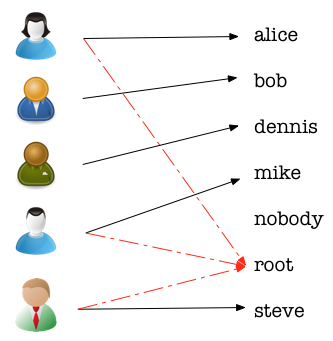
\includegraphics[width=.3\textwidth]{06/pics/user-mapping}}
	\subfloat[Group mappings]{\label{fig:multi-user:goup-mappings}
			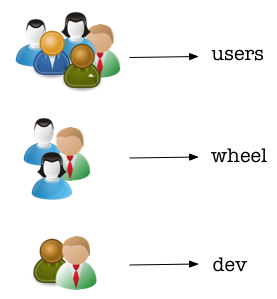
\includegraphics[width=.3\textwidth]{06/pics/user-groups}}
	\subfloat[Groups to machines mappings]{\label{fig:multi-user:goup-machine}
			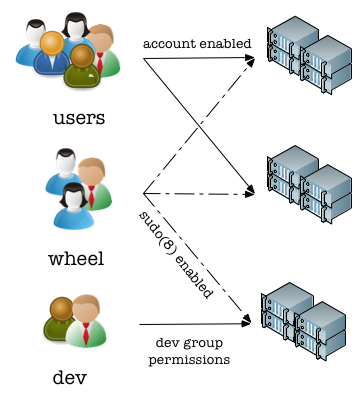
\includegraphics[width=.3\textwidth]{06/pics/groups-machines}}
	\caption[User Mappings]{The set of users mapping to the
			set of account names is neither bijective (or
			``one-to-one''), nor surjective (or ``onto''):
			some accounts are not used by an actual user,
			while others may be used by more than one user.
			Users are associated with local groups on a given
			host, and group membership may imply specific
			privileges across a set of hosts.
			\label{fig:multi-user:mappings}}
\end{figure}



\section{Groups of Users}
\label{multi-user:groups}

In addition to different {\em types} of users, we can
also identify different {\em groups} of users.
Privilege separation is a fundamental best practice in
the area of system administration: every user should
be given exactly the level of access they require,
with elevated or superuser privileges being
particularly strictly controlled.  But even outside
this special group, there are a number of users who
need to share resources with one another.  The nature
of the environment you are in plays an important role
here, as (implicit) trust or lack thereof create
vastly different use cases.  For the purposes of this
discussion, let us define a group of users as a number
of people who are either collaborating in some
capacity -- meaning they will wish to share read and
write access to certain resources -- or require
similar execute privileges, for example to start,
stop, or otherwise control a specific service.

In a small commercial environment, such as a start-up,
the good will and intent to collaborate for all users
of your systems is implied.  In such environments all
users do frequently require the same or at least
similar access to all systems, as responsibilities are
shared and job duties overlap.  As a result, you will
find few distinct groups here, and getting access to
one system tends to simultaneously get you (the same
broad) access to all systems.

As the environment grows in size, however, you will
find that you need to group accounts more carefully.
For example, all developers on a given software
project require access to systems on which to build
the software, write access to the central source
revision control repository and the like, and so are
grouped together; they do not require -- nor should
they have -- access to the systems processing credit
card payments or which contain payroll information.

In even larger companies, you may find that groups
sharing access to the same set of servers may have
competing resource requirements, even if we assume
that every user has been given an account for the
ultimate benefit of the organization at large. In
addition, the larger your organization grows and the
more users you have, the higher the risk of any one
account getting compromised becomes.  Recall our
earlier discussion of well-defined and documented
policies in Section
\ref{documentation:types:policies}; it is no surprise
to find a requirement for very specific access
policies, that spell out in detail who should be
granted what level of access on the one hand and for a
complete audit trail of who was given said access on
the other. \\

In contrast to these use cases, now consider the
different groups of users present in an academic
environment, such as a large university.  Access to
computing resources is made available to students,
faculty, staff, and possibly visiting researchers.
Even disregarding any outside compromise, you have at
times almost directly conflicting privacy
requirements: students should not be able to access
faculty resources or files (and yet may have an
explicit interest in doing so!), but students working
as teaching or faculty assistants sometimes should;
student homework assignments done on shared servers
should not prevent research jobs from running; faculty
may collaborate with each other on some projects, with
outside researchers on others.

Finally, if you are maintaining public systems for an
Internet Service Provider (ISP), you may find yourself
trying to manage hundreds or thousands of completely
unrelated user accounts with little to no
collaboration amongst them.


Group definitions exist in every organization, and are
often drawn outside the system administrator's
purview; it is not uncommon for computer systems to
inherit a group structure by mapping the
organization's functional hierarchy into different
user groups.  However, sooner or later you will run
into limitations and require more fine-grained
control.  A careful analysis of the different types of
users, the different groups based on requirements and
needs, and a directory service that allows you to
easily create (possibly intersecting) sets of users
are needed to allow your systems to grow with and
adapt to the needs of whichever type of environment
you are in.  We will get back to this concept of
grouping users and mapping them to similarly grouped
sets of hosts in our next chapter.

\begin{experience}
{\bf All users are equal...} \\

In almost every organization, there are a few users
who have {\tt root} who... shouldn't: there's the
ex-system administrator, who now works in a different
area but who occasionally is called upon when tribal
knowledge from the olden days is required; there's the
competent software developer who always needed special
resources and who finally managed to convince one of
the system administrators to let him have superuser
access to fix his own systems; there's the CEO who
simply ``requires'' superuser access to all machines,
even though the last time he opened a terminal was 10
years ago when he updated the single web server of his
then-fledgling start-up. \\ [10pt]

And then there's the start-up founder, who not only
routinely tinkers with the OS kernel and system
configurations, but oversees the hardware allocation
requests in what has become an Internet giant with
tens of thousands of hosts in data centers across the
globe: \\ [10pt]

While working at Yahoo!, I continually tried to keep
small the number of people whose accounts were
included in the OS images.  As an initially large
number was slowly reduced (often only after many
discussions, assurances of emergency failover
procedures, and arguments), I finally had to tell
David Filo\index[names]{Filo, David} (one of Yahoo!'s
founders) that I intended to remove his account as
well.  After a few discussions, assurances of
emergency failover procedures, and arguments, we
eventually agreed to have it removed from the OS
images, but to let our configuration management
systems add it as necessary.  To the best of my
knowledge, Filo, as he is known to all employees,
still logs into production servers to analyze and
challenge current resource usage whenever engineers
request new hardware, and he still traces and fixes
kernel bugs that require him to have access to most,
if not all, systems.  \\[10pt]

Every system administrator I know has a similar story
to tell; they frequently end with ``Well, he doesn't
{\em need} access, but he's the boss, so...''. \\
[10pt]

{\em Some users are more equal than others.}
\end{experience}

\section{User Authentication}
\label{multi-user:authentication}
\index{authentication}

We mentioned earlier (albeit somewhat tersely) that
the system authenticates the user at login time.
Seeing how this is a rather important aspect of a
multi-user system, let us spend a little bit of time
to make sure we understand what exactly happens.  As
we will discuss in more detail in Chapter
\ref{chap:security}, when we are authenticating a
user, we are ensuring that user is who they claim to
be.  More precisely, we are verifying that whoever is
identifying themselves as user ``alice'' can in fact
provide the credentials which we assume only Alice to
have access to.\footnote{Unlike the system
administrator in charge, the computer does not care if
Alice gives her credentials to Bob and allows him to
log in as her.}

{\em Authentication} (frequently referred to as {\em
AuthN}) is the act of providing a proof of identity,
not a proof of {\em authorization} ({\em AuthZ}).
Although frequently entangled, the former only answers
the question ``Are you really who you say you are?'',
while the latter concerns itself with the question
``Are you allowed to perform this action?''.  There
are many different ways of providing a proof of
authentication; we generally divide them into the
following three classes\footnote{Cynical information
security professionals, always happy to point out
weaknesses in any system, like to refer to these
categories as ``something you forgot, something you
lost, something you stopped being''.}:

\begin{itemize}
	\item {\em something you know}, for example a password
	\item {\em something you have}, for example a
		physical key or a hardware token
	\item {\em something you are}, a biometric
		factor, such as e.g. a fingerprint
\end{itemize}

Each authentication method has its own strengths and
weaknesses, with usability and convenience being
important factors upon the final security they may
provide:  passwords that are easy to remember are also
easy to guess or crack, physical tokens can be lost or
stolen, and biometric factors are near impossible to
replace or change in case of a compromise.

In many cases, it is desirable to combine some of
these authentication methods to yield the desired
level of security and usability.  So-called
``two-factor authentication'' or {\em
2FA}\index{authentication!2FA} has
recently become a popular protection mechanism used by
many internet sites: in order to gain access to a
service, the user needs to provide e.g. a password
({\em something you know}) as well as a code generated
by an app on their smartphone (the phone thus being
{\em something you have}).  It is entirely possible --
and at times desirable -- to add more factors or vary
combinations of factors, which is why the more general
term ``multi-factor
authentication''\index{authentication!multi-factor}
(MFA) is more precise.

Lastly, let us note that even though we frequently
only consider authentication of one party, {\em mutual
authentication}\index{authentication!mutual} is an
often desired or even required property of a secure
system:  when a user logs into a system, the system
wishes to authenticate the user, but the user also
needs to have assurance that the system they are
logging in to is the system they think it is.

\subsection{Authentication Examples}
\label{multi-user:authentication:examples}

To illustrate the many different ways we may use or
encounter authentication in our day to day operations,
let us look at a few examples:

\begin{lstlisting}[float,basicstyle=\scriptsize,label=code:password-login,caption={[Password
authentication on the console]Password authentication
on the system console on a NetBSD server.}]
NetBSD/amd64 (SERVER) (console)

login: jschauma
password: *********************************
NetBSD 7.0.2 (SERVER) #2: Tue Jan 24 02:33:13 EST 2017

Welcome to NetBSD!
hostname$
\end{lstlisting}

Listing \ref{code:password-login} illustrates the most
simple example: password authentication on the system
console of a NetBSD server.  The user provides their
username and password; if the password matches (see
below), the user is logged in.

\begin{lstlisting}[float,basicstyle=\scriptsize,label=code:ssh-login,caption={[SSH
key authentication]An example of mutual authentication
by way of SSH keys.}]
$ ssh -i ~/.ssh/mykey server
The authenticity of host 'server (192.0.2.12)' can't be established.
ECDSA key fingerprint is 19:af:35:01:0b:2a:ee:3d:30:0f:69:11:cc:55:7c:20.
Are you sure you want to continue connecting (yes/no)?  yes
NetBSD 7.0.2 (SERVER) #2: Tue Jan 24 02:33:13 EST 2017

Welcome to NetBSD!
hostname$
\end{lstlisting}

Listing \ref{code:ssh-login} shows another method of
authentication so frequently used that we hardly ever
think about it.  Here, we see asymmetric key
cryptography\index{cryptography!asymmetric} as a means
of authentication, effectively using a {\em something
we have} (a private SSH key).  But note that at the
same time, the server also offers {\em us} a way to
authenticate {\em it}: the SSH hostkey fingerprint
presented on the first connection allows us to verify
that the server is in fact the one we intended to
connect to.  If we know the server's expected hostkey
fingerprint (which itself is derived from the private
hostkey that presumably nobody else would have access
to), then we can compare and match them, thereby
authenticating the server.\footnote{Unfortunately, the
distribution of known hostkey fingerprints and
changing identities in a large scale environment have
lead most people to blindly accept any hostkey
fingerprint presented.  Doing so is an example of {\em
\gls{tofu}}\index{Trust on First Use}.  We will get
back to this problem in later chapters.}

\begin{lstlisting}[float,basicstyle=\scriptsize,label=code:krb-login,caption={[Kerberos authentication]Mutual authentication via a central Kerberos service.}]
$ kinit
Password for jschauma@DOMAIN: ********************************
$ klist
Ticket cache: /tmp/krb5cc_ttypa
     Default principal: jschauma@DOMAIN

     Valid starting     Expires            Service principal
     02/13/17 13:50:21  02/13/17 21:50:20  krbtgt/KDC@DOMAIN
$ ssh somehost
somehost$
\end{lstlisting}

Listing \ref{code:krb-login} illustrates the use of a
central authentication service by way of the
Kerberos\index{Kerberos} protocol.  Here, we are
authenticating ourselves to the central service using
a password ({\em something we know}).  We then use a
time-based token (a ``ticket'' in Kerberos lingo, i.e.
{\em something we (now) have}) to authenticate
ourselves to the server we wish to access.  At the
same time, the Kerberos network authentication
protocol also takes care of authenticating the server
to us.  This setup thus includes multiple
authentication methods as well as an example of mutual
authentication.

\begin{lstlisting}[float,basicstyle=\scriptsize,label=code:sshca-login,caption={[SSHCA
and MFA example]An example of very strong
authentication: the use of a certificate authority,
combined with a password and multiple physical
tokens.}]
localhost$ ssh sshca
YubiKey for `jschauma': ********************************
Password: ********************************
localhost$ ssh-add -l
2048 SHA256:TzwuHGc5BKBe+VJSnGoVyh92J8XKBUkaL7MGQn8ML0Y (RSA)
2048 SHA256:TzwuHGc5BKBe+VJSnGoVyh92J8XKBUkaL7MGQn8ML0Y (RSA-CERT)
localhost$ ssh somehost
Duo two-factor login for jschauma

Enter a passcode or select one of the following options:

 1. Duo Push to XXX-XXX-0712
 2. Phone call to XXX-XXX-0712
 3. SMS passcodes to XXX-XXX-0712

Passcode or option (1-3): 1
Success. Logging you in...
Last login: Thu Jan 26 17:39:30 2017 from 10.1.2.3

somehost$
\end{lstlisting}

Listing \ref{code:sshca-login} finally illustrates the
use of several strong factors combined with time-based
access credentials to form a particularly strong
example of authentication.  Here, we are making use of
a Certificate Authority (CA)\index{certificate
authority} for use with SSH to issue short-lived
access credentials.  In order to receive such a
certificate, the user must first authenticate to the
{\tt sshca} service, which requires both a password
(again: {\em something we know}) as well as a
cryptographic One-Time Password
(OTP)\index{passwords!one-time} generated by a
hardware token ({\em something we have}).  In addition
to the client certificate we received from the CA, the
server we are finally accessing also implements
another form of two-factor authentication, offering to
send a message to the user's cell phone and requiring
an interactive acknowledgement.  If the cell phone in
question requires a fingerprint to unlock, then we are
even adding a biometric factor ({\em something we
are}).  Phew, that is one tough system to access!

\subsection{The Problem with Passwords}
\label{multi-user:authentication:passwords}

Despite the variety of authentication methods
available, password authentication remains the lowest
common denominator and is worth looking at in a little
bit more detail.

More often than not, the credentials used to
authenticate at login time are simply a password of
often pitiful complexity.  Much like you may have not
let your sister (or her friends) climb into your tree
house unless they knew the secret passphrase, the Unix
system will not let you log in without you entering
the correct string of characters.

It is important to understand at this point that the
Unix system does not actually compare the string you
entered to the string it has stored in a database, but
that instead it operates on password {\em hashes}.
That is, the string you entered (together with a few
bits of additional data known as the {\em salt}) is
transformed via a one-way function that produces a
fixed-length string of (different) characters, which
are then stored and compared against at the time of
authentication.  Since this transformation is a {\em
one-way} function, it is impossible for anyone to
reproduce the original password from the hash -- an
important cryptographic property of the function used.
If this password hash matches the one on record,
access is granted, and you are logged in.  From that
moment on, regular Unix semantics and permissions will
apply to decide whether or not access to a given
resources (e.g. the ability to write to a file) is
granted.

Passwords are an easy and convenient way for users to
authenticate to a system.  However, there are quite a
few drawbacks that it is important to be consciously
aware of.

As noted above, we do not actually store clear text
passwords in a database, as this would mean that
anybody (and any process) able to access this database
had access to all users' passwords.  Instead, the
use of a hash ensures that even using a privileged
account, we cannot see the users' clear text
passwords.  Still, we wish to protect the password
hashes from prying eyes, which is why our Unix
systems no longer store them in the world-readable
{\tt /etc/passwd} database, but instead in a separate,
protected file (such as {\tt
/etc/master.passwd}\index{\tt /etc/master.passwd} on
BSD derived systems or {\tt /etc/shadow}\index{\tt
/etc/shadow} on many System V derived Unix
versions).

But, and this is one of the problems when using
passwords for local authentication, this data has to
exist on all the hosts a user wishes to log in on.
That, in turn, means that if a single host in the
environment is compromised, the attacker gets their
hands on {\em all} users' password hashes.  Once
retrieved, they can then perform so-called offline
dictionary attacks on the password hashes or look them
up in widely available {\em rainbow
tables}\index{rainbow tables}, large pre-computed
mappings of common strings to their hashes.

The solutions, or rather, the efforts to at least
partially address these issues include the use of a
password {\em salt}\index{salt}, the previously
mentioned small amount of data added to the user's
password prior to the application of the hash
function, thereby yielding a different hash on
unrelated systems despite the password being the same
and thus defeating simple rainbow table look ups.

Another approach used frequently is to not make the
password hash locally available on each host and
instead rely on an authentication system where the
actual password hashes and additional user
information is stored in a central place and is
accessed over the network.  The {\em
\gls{ldap}\index{LDAP}} is an example of this
approach.  However, it should be noted that the
benefits of a central location of this information
carries a certain prize, as well: if the host(s)
providing this service becomes unavailable, thousands
of hosts can become unusable or see debilitating
errors.  This problem can of course be defined in a
more general statement: as an environment increases in
size, relying on a central service poses an increasing
risk of becoming a {\em Single Point of
Failure}\index{Single Point of Failure} (often
abbreviated as ``\glslink{spof}{SPOF}''), while
distributing data across thousands of servers poses
its own data replication and synchronization
challenges while simultaneously increasing the
probability of it being compromised.

What's more, passwords are an inherently insecure
means of authentication, largely due to human nature:
most people are rather terrible at remembering complex
passwords (which are harder for computers to crack)
and hence tend to use and reuse across different sites
a small set of a simple passwords This means that
accounts on your systems may get compromised by
password leaks in another, completely different and
independent environment!

Many solutions or improvements to this dilemma exist,
ranging from multi-factor authentication protocols to
randomly generated passwords stored and managed by
specific password management tools.  We will discuss
some of these in our chapter on security later in the
book.

\subsection{Sharing {\tt root}}
\label{multi-user:authentication:shared-root}

As noted in Section \ref{multi-user:types}, the {\tt
root} account is commonly shared, meaning multiple
people know the password to authenticate as the
superuser.  This, however, poses a number of problems.
When a system administrator leaves the organization,
the {\tt root} password needs to be changed, all
systems need to be updated with the new password hash,
and the new password has to be communicated to all
members of the team.  Despite many best practices of
sharing or storing shared secrets like this, the more
people who require said access, the larger the risk of
accidental exposure of the password or its hash.

Secondly, since the {\tt root} account is a {\em
system} account, it may not be included in any central
user directory (such as your \gls{ldap} service), and
instead be managed either via your configuration
management system, or your OS image.  This may lead to
the password hash being available in additional
places, such as the configuration management's
repository or the OS image build system.  Again: the
more places such important access credentials are
stored, the more likely it is that they can be
accessed by unauthorized parties.

Finally, by mapping multiple people to a single
account you lose an important audit-trail: no longer
is it possible to identify who performed a given task;
all we can do is identify a (possibly large) group of
people who could have done so.  Given the powers of
the superuser account, this is particularly
bothersome.

It is common best practice to disable logins from {\tt
root} over the network\footnote{It is also possible to
completely disable the {\tt root} account, though that
may have implications on your ability to recover the
system without physical access in the case of a severe
failure.}, requiring users to first log in with their
usual account, and then to use the {\tt
su(1)}\index{\tt su(1)} or {\tt sudo(8)}\index{\tt
sudo(8)} utility to perform certain actions with
elevated privileges. Since this tool logs all
invocations, we nicely solve the problem of the
missing audit trail; in addition, we gain much finer
grained control of what access is given to which
users.

Note, however, that this solution is no panacea: it is
easy to fall into a false sense of security when
restricting superuser privileges to a few explicit
commands while forgetting that many of these commands
allow a skilled user to invoke or otherwise trick the
system into executing other, non-sanctioned
commands.\footnote{Most Unix editors, for example,
allow a user to invoke a shell; dynamically linked
executables can be tricked into loading custom
libraries; the possibilities to exploit access to a
small number of tools running with superuser
privileges are too numerous to account for.}  As a
general rule of thumb, you should consider the use of
{\tt sudo(8)} primarily for its audit-trail
capabilities and only grant its use to trusted users.

Secondly, this approach only works on actual server
operating systems.  Networking equipment, such as
switches, routers, or load balancers, where the {\tt
TACACS+}\index{\tt TACACS+} and {\tt
RADIUS}\index{\tt RADIUS} remote authentication
protocols allow well-defined control of remote access
do, for the most part, still follow an all-or-nothing
access model locally.  The access credentials for the
privileged accounts on these devices (as example might
be the ``enable'' password, used to enter privileged
mode on a router or switch) need to be managed and
shared with the same care that a {\tt root} password
would be.

\section{Summary}
\label{multi-user:summary}

Even though taken for granted nowadays, the nature of
a {\em multi-user} system has had from the beginning a
number of important implications for overall system
security and operational procedures.  The impact of
these implications grows near exponentially as your
environment scales up, which is why we make a point of
identifying them explicitly in this chapter.

Users fall into a number of well-defined categories,
or {\em types} of users.  In particular, we
distinguish for good reasons between user accounts
used by actual humans and so-called system accounts.
Different users (of either kind) have at times
conflicting requirements and impose very specific
trust models on the environment.  Access privileges
need to be defined and enforced, and authentication
methods need to be considered.  We briefly mentioned
passwords as the most common form of authentication
and noted a few of the problems associated with them;
we also covered some of the implications of sharing
{\tt root} access with your peers.

More generally speaking, though, we looked at what it
means for a system to support multiple users.  System
administrators with experience managing deployments in
diverse environments are able to recognize and apply
these general rules:

\begin{itemize}
	\item {\em All users are equal.}  We need to be able to
		accomodate different use cases and equally enable many
		different types of requirements.  All groups of users
		should be treated with the same professionalism and their
		needs appropriately addressed.
	\item {\em Some users are more equal than others.}  While all
		users' needs should be addressed, there are, in any
		system, some users who have more specific requirements;
		who need certain elevated privileges; whose computing
		demands exceed those of others.
	\item {\em All users are to be given precisely the access rights
		they need, but no more.}  The principle of least privilege
		needs to be rigorously applied, as any one account may
		become compromised, and the possible damage deriving from
		this scenario needs to be limited as much as possible.
	\item {\em Trust does not scale.}  When building your
		infrastructure, remember that while you may trust all
		users in your organization {\em today}, you will
		eventually grow to a size where this no longer holds.  It
		is near impossible to later on put in place restrictions
		on users' privileges, just as it is to anticiapate the
		possibly sudden departure of trusted employees.
	\item {\em You will always face tradeoffs.}  No matter which
		authentication mechanism you choose, there are downsides.
		Eliminating single points of failure may increase your
		infrastucture's complexity or increase the risk of
		exposure of confidential information.  (This holds for
		many other aspects of system administration, too, but the
		impact may be most obvious when it comes to
		authentication of users.)
\end{itemize}

When you manage a sufficiently large or diverse group
of systems, you will learn to abstract individual
users (and their requirements) into more conceptual
{\em groups of users}.  These groups may then be
translated to access privileges on a given host, or,
as you scale up your environment, to mappings of
privileges to {\em sets of hosts}.

Controlling only a few hundred machines, it is easy to
think in terms of individual hosts.  However, today's
Internet giants tend to operate by utilizing tens or
hundreds of thousands of hosts.  At this scale,
services are defined not by which individual machines,
but by which {\em datacenter} handles the requests.
Individual hosts become irrelevant, even though access
control, by and large, still follows the same model,
even if operating on a different scale.

Due to this shift in scale, a distinct trend away from
managing user access on an individual host basis and
instead shifting towards a {\em Service
Orchestration}\index{Service Orchestration} model has
formed in the last couple of years.  In this world,
interactive logins to any single host are unnecessary
and imply a systemic failure, as unavailable hosts
should automatically be taken out of a
production-serving rotation and overall load be
distributed to the remaining, working hosts.

Services are run as so-called system accounts
unassociated with actual users.  Nevertheless, regular
multi-user semantics apply.  The principles of how
access to any given resource is granted, how services
(or users) are authenticated, and how a clear
separation of privileges provides the foundation for
overall system security is not different when applied
to user accounts that end up being mapped to humans
versus those that are not.  \\

A multi-user system implies the existence of a
privileged account, which, by necessity, is shared
amongst multiple people.  The fact that this account
is also -- by definition -- a system account embodies
the paradoxical complexity of managing {\em all} user
accounts (whether or not they may be mapped to people
or service roles).  The only way to retain a modicum
of sanity when managing these many-to-many mappings of
privilege in a large environment is a clear definition
of host and user access groups.  As we will see in the
following chapter, creating and operating on these
sets of resources in the abstract is best done using a
configuration management system.

Looking towards the future (as we will in Chapter
\ref{chap:future}) -- and catching up a bit with
developments since I first started writing this
chapter back in 2012 -- we should also note that as
the industry moves further towards more ephemeral
systems, such as through the use of containers and
virtualization technologies, the overall headache of
managing local user accounts may well be a thing of
the past: systems are defined in a descriptive way and
spun up or torn apart as needed.  Nevertheless, as
experienced system administrators, we are well aware
that new headaches may well lie hidden here, and the
{\em concept} of authenticated access by multiple
users (for humans and services alike) continue to
apply.

Thus, the burden of {\em identifying} the proper
access model, however, remains with the system
administrators.  Let's make sure that we understand
the implications of multi-user access on all of our
systems as we do!

\vfill
\pagebreak

\chapter*{Problems and Exercises}
\addcontentsline{toc}{chapter}{Problems and Exercises}
\section*{Problems}
\addcontentsline{toc}{section}{Problems}

\begin{enumerate}

\item Review the {\tt passwd(5)}\index{\tt
passwd(5)} manual page and make sure you understand
what each field is used for.  Is this password
database used on the systems you have access to, or is
authentication done by way of a central system, for
example via \gls{ldap}?  If so, what additional
information can you find in this system?

\item
Review the accounts present on your systems.  How many
of these are system accounts, and how many are user
accounts?  What different types of users can you
identify?  Are there any role accounts?

\item
Review the different groups present on your systems.
Identify the groups with the most users in it and what
it is used for.  What resources on the system are
accessible only by belonging to a specific group?

\item
Identify whether or not {\tt sudo(1)} is used on the
systems you have access to.  Can you find out which
users have which privileges?  Which, if any, commands
can you think of that might be dangerous to allow
untrusted users to invoke?  Try to think of
non-obvious ways to circumvent the given restrictions.

\item
Compare the default {\tt /etc/passwd} file on a few
different Unix versions.  What kinds of differences do
you notice?  What kinds of accounts are present on one
but not another?

\item
Consider some of the online services you use.  What
types of authentication do they require?  Which offer
multi-factor authentication?  What kinds of factors do
they use?

\item
Search the Internet for a list of the most popular
passwords in use (such as, not surprisingly,
``password'').

\begin{enumerate}
\item
Generate hashes for each password using the following
digest algorithms: DES (as used by the Unix {\tt
crypt(3)}\index{\tt crypt(3)} family),
MD5\index{MD5} and SHA1\index{SHA1}.  Can you find the
resulting strings in any rainbow tables on the
Internet?

\item
Repeat the previous exercise, but add a salt to the
password.  What do you notice about the results?
\end{enumerate}

\item
Write a tool to create a new account on a remote
system.  The tool should take as input the username of
a local account; the account on the remote system
should be identical with regards to UID, GID,
supplementary groups, login shell etc. to that on the
local system.
\end{enumerate}

\pagebreak

\bibliographystyle{plainnat}
\begin{thebibliography}{99}

\bibitem{multi-user:frisch} \AE leen Frisch, {\em Essential System
Administration}, O'Reilly Media, 2002

\bibitem{multi-user:burgess-principles}Mark Burgess, {\em Principles of
Network and System Administration}, Wiley \& Sons, 2nd Edition, 2004

\bibitem{multi-user:nemeth-unix-handbook}Evi Nemeth, Garth Snyder, Trent
R. Hein, Ben Whaley {\em UNIX and Linux System Administration Handbook},
4th Edition, Prentice Hall, 2010

\end{thebibliography}
